\documentclass[12pt,a4paper]{article}
\usepackage{fontspec}
\XeTeXlinebreaklocale "th"
\XeTeXlinebreakskip=0pt plus 1pt
\defaultfontfeatures{Ligatures=TeX}
\setmainfont[
  Path={fonts/TH Sarabun PSK V-1/},
  Extension=.ttf,
  UprightFont={*},
  BoldFont={* Bold},
  ItalicFont={* Italic},
  BoldItalicFont={* BoldItalic}
]{THSarabun}
\setmonofont{Latin Modern Mono}
\usepackage{amsmath,amssymb,mathtools}
\usepackage{graphicx,float,caption,xcolor}
\usepackage{geometry,booktabs,tabularx,array}
\usepackage{tikz}
\usetikzlibrary{arrows.meta,positioning,calc,shapes.geometric}
\usepackage{enumitem}
\usepackage[hidelinks]{hyperref}
\geometry{top=0.78in,bottom=0.72in,left=0.82in,right=0.82in}
\setlength{\parindent}{1.5em}
\setlength{\parskip}{0pt}
\linespread{1.05}
\emergencystretch=2em
\renewcommand{\arraystretch}{1.12}
\setlength{\tabcolsep}{4pt}
\captionsetup{font=normalsize,labelfont=bf}
\renewcommand{\figurename}{รูปที่}
\renewcommand{\tablename}{ตารางที่}
\setlist[enumerate]{leftmargin=2.2em,itemsep=0.15em,topsep=0.25em}
\setlist[itemize]{leftmargin=2.0em,itemsep=0.15em,topsep=0.25em}
\pagestyle{plain}
\definecolor{navy}{RGB}{24,54,93}
\definecolor{teal}{RGB}{0,110,112}
\definecolor{lightblue}{RGB}{238,245,250}
\definecolor{lightgreen}{RGB}{238,248,241}
\newcommand{\pu}{\ensuremath{\,\mathrm{pu}}}
\newcommand{\hz}{\ensuremath{\,\mathrm{Hz}}}
\newcommand{\second}{\ensuremath{\,\mathrm{s}}}
\newcommand{\sci}[2]{\ensuremath{#1\times10^{#2}}}
\newcommand{\templateheading}[1]{\vspace{0.55em}\noindent{\fontsize{18}{22}\selectfont\bfseries #1}\par\vspace{0.25em}}
\newcommand{\templatesubheading}[1]{\vspace{0.35em}\noindent{\fontsize{16}{20}\selectfont\bfseries #1}\par\vspace{0.15em}}
% Generated by generate_ieee14_gfm_lock_comparison. Do not edit.
% Every number the comparison section prints comes from here, so the prose cannot drift
% from the runs. Arm keys: adaptive, pinned_gfm1, pinned_gfm2, pinned_gfm4, locked_gfl

\newcommand{\ArmAdaptiveLabel}{adaptive}
\newcommand{\ArmAdaptiveHorizon}{250.000}
\newcommand{\ArmAdaptiveConverged}{1}
\newcommand{\ArmAdaptiveReclose}{159.2397}
\newcommand{\ArmAdaptiveGfmMax}{4}
\newcommand{\ArmAdaptiveFailure}{--}
\newcommand{\ArmAdaptiveSamples}{4990}
\newcommand{\ArmAdaptiveRejected}{135}
\newcommand{\DfAdaptiveSGtrip}{0.7587}
\newcommand{\SetAdaptiveSGtrip}{0.0041}
\newcommand{\DfAdaptiveLoadstep}{1.0035}
\newcommand{\SetAdaptiveLoadstep}{0.3753}
\newcommand{\DfAdaptiveFault}{1.1386}
\newcommand{\SetAdaptiveFault}{0.3753}
\newcommand{\DfAdaptiveLinetrip}{0.3764}
\newcommand{\SetAdaptiveLinetrip}{0.3503}
\newcommand{\DfAdaptiveRestorereclose}{1.1612}
\newcommand{\SetAdaptiveRestorereclose}{0.0130}
\newcommand{\ArmPinnedgfmOneLabel}{pinned 1 GFM}
\newcommand{\ArmPinnedgfmOneHorizon}{250.000}
\newcommand{\ArmPinnedgfmOneConverged}{1}
\newcommand{\ArmPinnedgfmOneReclose}{151.4244}
\newcommand{\ArmPinnedgfmOneGfmMax}{1}
\newcommand{\ArmPinnedgfmOneFailure}{--}
\newcommand{\ArmPinnedgfmOneSamples}{3232}
\newcommand{\ArmPinnedgfmOneRejected}{542}
\newcommand{\DfPinnedgfmOneSGtrip}{0.5312}
\newcommand{\SetPinnedgfmOneSGtrip}{0.0113}
\newcommand{\DfPinnedgfmOneLoadstep}{1.4478}
\newcommand{\SetPinnedgfmOneLoadstep}{1.2214}
\newcommand{\DfPinnedgfmOneFault}{1.4979}
\newcommand{\SetPinnedgfmOneFault}{1.2296}
\newcommand{\DfPinnedgfmOneLinetrip}{1.2325}
\newcommand{\SetPinnedgfmOneLinetrip}{1.1426}
\newcommand{\DfPinnedgfmOneRestorereclose}{1.1736}
\newcommand{\SetPinnedgfmOneRestorereclose}{0.0210}
\newcommand{\ArmPinnedgfmTwoLabel}{pinned 2 GFM}
\newcommand{\ArmPinnedgfmTwoHorizon}{250.000}
\newcommand{\ArmPinnedgfmTwoConverged}{1}
\newcommand{\ArmPinnedgfmTwoReclose}{149.9191}
\newcommand{\ArmPinnedgfmTwoGfmMax}{2}
\newcommand{\ArmPinnedgfmTwoFailure}{--}
\newcommand{\ArmPinnedgfmTwoSamples}{3183}
\newcommand{\ArmPinnedgfmTwoRejected}{321}
\newcommand{\DfPinnedgfmTwoSGtrip}{0.3489}
\newcommand{\SetPinnedgfmTwoSGtrip}{0.0001}
\newcommand{\DfPinnedgfmTwoLoadstep}{0.7839}
\newcommand{\SetPinnedgfmTwoLoadstep}{0.7123}
\newcommand{\DfPinnedgfmTwoFault}{0.8255}
\newcommand{\SetPinnedgfmTwoFault}{0.7126}
\newcommand{\DfPinnedgfmTwoLinetrip}{0.7135}
\newcommand{\SetPinnedgfmTwoLinetrip}{0.6422}
\newcommand{\DfPinnedgfmTwoRestorereclose}{0.6634}
\newcommand{\SetPinnedgfmTwoRestorereclose}{0.0209}
\newcommand{\ArmPinnedgfmFourLabel}{pinned 4 GFM}
\newcommand{\ArmPinnedgfmFourHorizon}{25.491}
\newcommand{\ArmPinnedgfmFourConverged}{0}
\newcommand{\ArmPinnedgfmFourReclose}{--}
\newcommand{\ArmPinnedgfmFourGfmMax}{4}
\newcommand{\ArmPinnedgfmFourFailure}{\texttt{adaptiveDtMin}}
\newcommand{\ArmPinnedgfmFourSamples}{819}
\newcommand{\ArmPinnedgfmFourRejected}{449}
\newcommand{\DfPinnedgfmFourSGtrip}{0.9898}
\newcommand{\SetPinnedgfmFourSGtrip}{--}
\newcommand{\DfPinnedgfmFourLoadstep}{--}
\newcommand{\SetPinnedgfmFourLoadstep}{--}
\newcommand{\DfPinnedgfmFourFault}{--}
\newcommand{\SetPinnedgfmFourFault}{--}
\newcommand{\DfPinnedgfmFourLinetrip}{--}
\newcommand{\SetPinnedgfmFourLinetrip}{--}
\newcommand{\DfPinnedgfmFourRestorereclose}{--}
\newcommand{\SetPinnedgfmFourRestorereclose}{--}
\newcommand{\ArmLockedgflLabel}{locked GFL}
\newcommand{\ArmLockedgflHorizon}{20.000}
\newcommand{\ArmLockedgflConverged}{0}
\newcommand{\ArmLockedgflReclose}{--}
\newcommand{\ArmLockedgflGfmMax}{0}
\newcommand{\ArmLockedgflFailure}{\texttt{noVoltageFormingSource}}
\newcommand{\ArmLockedgflSamples}{43}
\newcommand{\ArmLockedgflRejected}{0}
\newcommand{\DfLockedgflSGtrip}{--}
\newcommand{\SetLockedgflSGtrip}{--}
\newcommand{\DfLockedgflLoadstep}{--}
\newcommand{\SetLockedgflLoadstep}{--}
\newcommand{\DfLockedgflFault}{--}
\newcommand{\SetLockedgflFault}{--}
\newcommand{\DfLockedgflLinetrip}{--}
\newcommand{\SetLockedgflLinetrip}{--}
\newcommand{\DfLockedgflRestorereclose}{--}
\newcommand{\SetLockedgflRestorereclose}{--}
\newcommand{\CommonWindowPinnedgfmOneBitIdentical}{1}
\newcommand{\CommonWindowPinnedgfmOneSamples}{42}
\newcommand{\CommonWindowPinnedgfmTwoBitIdentical}{1}
\newcommand{\CommonWindowPinnedgfmTwoSamples}{42}
\newcommand{\CommonWindowPinnedgfmFourBitIdentical}{1}
\newcommand{\CommonWindowPinnedgfmFourSamples}{42}
\newcommand{\CommonWindowLockedgflBitIdentical}{1}
\newcommand{\CommonWindowLockedgflSamples}{42}
\newcommand{\CommonWindowSplit}{20.000}
\newcommand{\CommonWindowAllBitIdentical}{1}
\newcommand{\CandTotal}{15}
\newcommand{\CandReady}{7}
\newcommand{\CandBestSet}{IBR3+IBR6}
\newcommand{\CandBestN}{2}
\newcommand{\CandBestOmega}{-0.56814}
\newcommand{\CandBestSingleOmega}{-0.32801}
\newcommand{\CandFullOmega}{-0.48291}
\newcommand{\CandReadyNOne}{4}
\newcommand{\CandTotalNOne}{4}
\newcommand{\CandReadyNTwo}{2}
\newcommand{\CandTotalNTwo}{6}
\newcommand{\CandReadyNThree}{0}
\newcommand{\CandTotalNThree}{4}
\newcommand{\CandReadyNFour}{1}
\newcommand{\CandTotalNFour}{1}

% Generated by generate_ieee14_report_scalars. Do not edit.
%
% PROVENANCE. Accepted values of output/diagnostics/ieee14_gfm_lock_compare_dcreal/adaptive_250s.mat.
% Produced by run_ieee14_gfm_lock_comparison, whose option set is the
% flagship driver's plus agsi_reference=true (opt-in, post-processing only).
% This cache is NOT bit-identical to the earlier delivered artifact, and no
% such claim is made for it: the DC-link closure changed under
% NUM-2026-08-20-01, so the trajectory legitimately differs. Compare it to
% the earlier cache by outcome, never by bit-identity.
% No value here is rounded, scaled, smoothed or otherwise altered.
%
% Regenerate with:  pf_init_paths; generate_ieee14_report_scalars(result_file="output/diagnostics/ieee14_gfm_lock_compare_dcreal/adaptive_250s.mat")

\newcommand{\NewRunEnd}{250.000}
\newcommand{\NewRunVMin}{0.036855}
\newcommand{\NewRunVMax}{1.523183}
\newcommand{\NewRunFMin}{58.838795}
\newcommand{\NewRunFMax}{61.138560}
\newcommand{\NewRunSubdivision}{0}
\newcommand{\NewRunDomainRejects}{584}
\newcommand{\NewRunResidual}{$9.9596\times10^{-9}$}
\newcommand{\NewRunReclose}{159.240}
\newcommand{\NewRunRecloseStatus}{SUCCESS}
\newcommand{\NewRunSyncDV}{0.008785}
\newcommand{\NewRunSyncDF}{$6.4601\times10^{-13}$}
\newcommand{\NewRunSyncDTheta}{5.015017}
\newcommand{\NewRunFirstRelease}{25.310}
\newcommand{\NewRunReleaseOne}{25.310}
\newcommand{\NewRunReleaseTwo}{146.247}
\newcommand{\NewRunReleaseThree}{152.390}
\newcommand{\NewRunReleaseFour}{--}
\newcommand{\NewRunAugmentOne}{22.052}
\newcommand{\NewRunAugmentTwo}{51.333}
\newcommand{\NewRunAugmentThree}{53.372}
\newcommand{\NewRunAugmentFour}{148.267}
\newcommand{\NewRunNRelease}{3}
\newcommand{\NewRunNAugment}{4}
\newcommand{\NewRunGfmMax}{4}
\newcommand{\NewRunSamples}{4990}
\newcommand{\NewRunRejectedSteps}{135}
\newcommand{\NewRunTerminalF}{60.000000}
\newcommand{\NewRunTerminalVMin}{0.9667}
\newcommand{\NewRunTerminalVMax}{1.0575}
\newcommand{\NewRunStepper}{adaptive}
\newcommand{\NewRunReselection}{NO\_FEASIBLE\_SG\_ON\_ONE\_STEP}

\graphicspath{{figures/}{figures/final_report_th/}{figures/presentation_pf_sssa_ts_gfm/}}

\begin{document}
\begin{titlepage}
\thispagestyle{empty}
\begin{center}
\vspace*{0.20in}
{\fontsize{26}{31}\selectfont\bfseries เอกสารสรุปวิชาโครงงาน\par}
\vspace{0.32in}
{\fontsize{18}{22}\selectfont\bfseries ชื่องานโครงงาน\par}
\vspace{0.12in}
{\fontsize{19}{24}\selectfont\bfseries
(ภาษาไทย) กรอบการสลับโหมดแบบอัตโนมัติระหว่าง Grid-Following และ Grid-Forming\\
สำหรับทรัพยากรที่เชื่อมต่อผ่านอินเวอร์เตอร์\par}
\vspace{0.13in}
{\fontsize{17}{21}\selectfont\bfseries
(ภาษาอังกฤษ) An Automatic Following/Forming Framework\\
for Inverter-Based Resources\par}
\vspace{0.38in}
{\fontsize{18}{22}\selectfont\bfseries สมาชิกผู้จัดทำ\par}
\vspace{0.08in}
{\fontsize{17}{21}\selectfont
1. Phichitchai Jueajan \hspace{0.35in} 66010569\\
2. Pakkapol Phdungdan \hspace{0.35in} 66010612\par}
\vspace{0.28in}
{\fontsize{18}{22}\selectfont\bfseries อาจารย์ที่ปรึกษา\par}
\vspace{0.08in}
{\fontsize{17}{21}\selectfont
1. Dr. Tossaporn Surinkaew\\
2. Prof. Dr. Issarachai Ngamroo\par}
\vfill
{\fontsize{15}{19}\selectfont
ภาควิชาวิศวกรรมไฟฟ้า คณะวิศวกรรมศาสตร์\\
สถาบันเทคโนโลยีพระจอมเกล้าเจ้าคุณทหารลาดกระบัง\par}
\vspace{0.15in}
{\fontsize{17}{21}\selectfont\bfseries ปีการศึกษา 2569\par}
\end{center}
\end{titlepage}
\templateheading{วัตถุประสงค์ของโครงงาน}
\begin{enumerate}
\item ศึกษาและพัฒนาสายงานคำนวณระบบไฟฟ้ากำลังที่เชื่อมโยงการไหลของกำลัง (Power Flow: PF) การวิเคราะห์เสถียรภาพสัญญาณขนาดเล็ก (Small-Signal Stability Analysis: SSSA) และการจำลองโดเมนเวลา (Time-Domain Simulation: TS) ภายใต้แบบจำลองเดียวกัน
\item พัฒนาแบบจำลองทรัพยากรที่เชื่อมต่อผ่านอินเวอร์เตอร์ (Inverter-Based Resources: IBR) ที่สามารถทำงานได้ทั้งโหมด Grid-Following (GFL) และ Grid-Forming (GFM)
\item พัฒนากลไก supervisor สำหรับสลับโหมด GFL/GFM อัตโนมัติตามสภาวะของระบบ โดยรักษาความต่อเนื่องของ state และกระแสที่จุดเชื่อมต่อ
\item ทดสอบกรอบการทำงานบนระบบ IEEE 14-bus ภายใต้เหตุการณ์รบกวนหลายชนิด และเปรียบเทียบผลกับนโยบายการควบคุมแบบอื่น
\end{enumerate}

\templateheading{ความสำคัญ และที่มาของปัญหาที่ทำโครงงาน}
ระบบไฟฟ้ากำลังในปัจจุบันมีสัดส่วนแหล่งพลังงานที่เชื่อมต่อผ่านอินเวอร์เตอร์เพิ่มขึ้นอย่างต่อเนื่อง เช่น ระบบผลิตไฟฟ้าจากพลังงานหมุนเวียนและระบบกักเก็บพลังงาน อุปกรณ์เหล่านี้มีพฤติกรรมแตกต่างจากเครื่องกำเนิดไฟฟ้าซิงโครนัส (Synchronous Generator: SG) ซึ่งเดิมเป็นแหล่งกำหนดแรงดัน ความถี่ และมุมอ้างอิงให้กับโครงข่าย

IBR แบบ GFL ทำงานโดยอาศัยแรงดันของโครงข่ายเป็นสัญญาณอ้างอิงผ่านวงจร Phase-Locked Loop (PLL) จึงเหมาะกับระบบที่มีแหล่งสร้างกริดอยู่แล้ว ในทางตรงกันข้าม GFM สามารถสร้างมุมและแรงดันอ้างอิงของตนเองได้ และจึงมีบทบาทสำคัญเมื่อระบบสูญเสีย SG หรือเข้าสู่สภาวะกริดอ่อน อย่างไรก็ตาม การกำหนดให้ IBR ทุกตัวทำงานเป็น GFM ตลอดเวลาไม่จำเป็นต้องให้ผลดีที่สุด และอาจเพิ่มความซับซ้อนของการควบคุมหรือทำให้การจำลองไม่ผ่านในบางสภาวะ
โครงงานนี้จึงเสนอกรอบการทำงานที่ให้ IBR เปลี่ยนบทบาทระหว่าง GFL และ GFM ตามความจำเป็นของระบบ โดยใช้ผลจาก PF, equilibrium, SSSA และสถานะที่ยอมรับแล้วจาก TS เป็นพื้นฐานในการตัดสินใจ การทดสอบหลักใช้ระบบ IEEE 14-bus ซึ่งประกอบด้วย SG ที่บัส 1 และ IBR จำนวน 4 ตัวที่บัส 2, 3, 6 และ 8 ดังรูปที่~\ref{fig:network}

\begin{figure}[H]
\centering
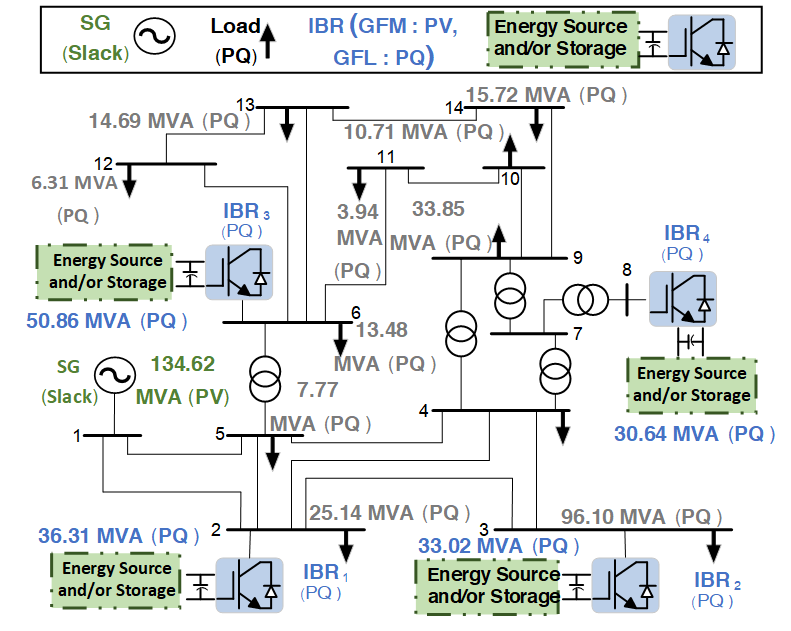
\includegraphics[width=0.78\textwidth]{123313.png}
\caption{ระบบ IEEE 14-bus ที่ใช้เป็นกรณีศึกษา โดยมี SG และ IBR แบบ GFL/GFM}
\label{fig:network}
\end{figure}

กรณีศึกษาถูกออกแบบให้เกิดการสูญเสีย SG การเปลี่ยนโหลด fault การปลดสายส่ง และการคืน SG เพื่อให้เห็นความจำเป็นของการเปลี่ยนบทบาทของ IBR อย่างชัดเจน หากไม่มีแหล่ง voltage-forming หลัง SG ถูกปลด ระบบจะไม่มีผู้ถือมุมอ้างอิงและตัวแก้สมการจะต้องหยุดแบบ fail-closed แทนการบังคับให้ผลลัพธ์ผ่าน

\clearpage
\templateheading{การดำเนินงานและผลงานที่ได้รับจากโครงงาน (โดยสังเขป) พร้อมภาพประกอบ}
\templatesubheading{1. พัฒนาสายงานคำนวณ PF--SSSA--TS ภายใต้แบบจำลองร่วม}
โครงงานพัฒนาตัวแก้สมการภายใน MATLAB โดยเริ่มจาก PF เพื่อหาจุดทำงานเริ่มต้น จากนั้นสร้างสมการเชิงอนุพันธ์--พีชคณิต (Differential-Algebraic Equations: DAE) สำหรับ equilibrium, SSSA และ TS ให้ใช้ residual และลำดับตัวแปรชุดเดียวกัน ลดความเสี่ยงจากการใช้แบบจำลองคนละชุดในแต่ละขั้นตอน

\begin{equation}
\dot{x}=f(x,y,u),\qquad 0=g(x,y,u)
\end{equation}
โดย $x$ คือ differential states, $y$ คือ algebraic states ของแรงดันบัส และ $u$ คืออินพุตหรือเหตุการณ์ของระบบ
\begin{figure}[H]
\centering
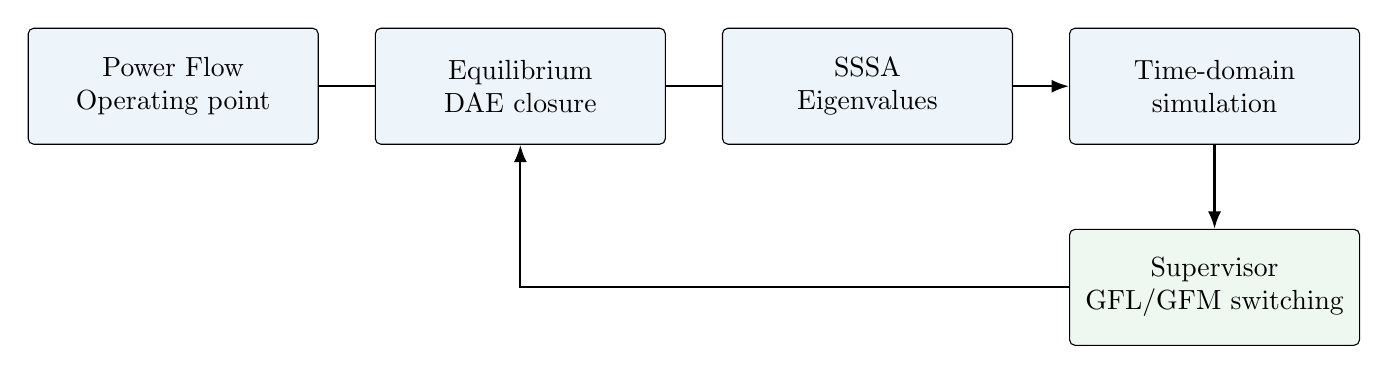
\begin{tikzpicture}[
  box/.style={draw=black,rounded corners=2pt,minimum width=1.45in,minimum height=0.58in,align=center,fill=lightblue},
  arr/.style={-{Latex[length=2.2mm]},thick}
]
\node[box] (pf) {Power Flow\\Operating point};
\node[box,right=0.28in of pf] (eq) {Equilibrium\\DAE closure};
\node[box,right=0.28in of eq] (sssa) {SSSA\\Eigenvalues};
\node[box,right=0.28in of sssa] (ts) {Time-domain\\simulation};
\node[box,below=0.42in of ts,fill=lightgreen] (sup) {Supervisor\\GFL/GFM switching};
\draw[arr] (pf)--(eq)--(sssa)--(ts);
\draw[arr] (ts)--(sup);
\draw[arr] (sup.west) -| (eq.south);
\end{tikzpicture}
\caption{ลำดับการคำนวณหลักของโครงงาน}
\end{figure}

ผล PF ของ IEEE 14-bus ลู่เข้าภายใน 5 รอบ Newton โดยมี mismatch สูงสุดประมาณ $6.34\times10^{-15}$ และสมดุลกำลังสอดคล้องกับโหลดรวมและการสูญเสียในสายส่ง การตรวจ SSSA ใช้ Schur complement เพื่อกำจัด algebraic variables และตรวจ eigenvalues จาก Jacobian ที่คำนวณด้วย finite difference ส่วน TS ใช้ implicit trapezoidal method และบังคับให้ทุกเหตุการณ์ลงตรงเวลา event ก่อนเปลี่ยน topology

\begin{table}[H]
\centering
\caption{ตัวอย่างผลตรวจสอบสายงานคำนวณหลัก}
\begin{tabularx}{0.94\textwidth}{@{}l l X@{}}
\toprule
หัวข้อ & ผลที่ได้ & ความหมาย \\
\midrule
PF IEEE 14-bus & Converged, 5 iterations & จุดทำงานเริ่มต้นมี residual ต่ำมากและสมดุลกำลังถูกต้อง \\
SSSA & Finite eigenvalues และ FD plateau ผ่าน & การ linearize มีความสอดคล้องเชิงตัวเลข \\
TS เทียบ PSAT & $\Delta f$ และ $\Delta V$ อยู่ในช่วง tolerance ที่กำหนด & trajectory ของตัวแก้ภายในสอดคล้องกับโปรแกรมอ้างอิงหลัก \\
Event handling & Exact event landing & ไม่มี time step เดียวคร่อม topology สองแบบ \\
\bottomrule
\end{tabularx}
\end{table}
\templatesubheading{2. พัฒนา IBR แบบสองโหมด GFL/GFM}
IBR แต่ละตัวใช้ plant ร่วม แต่มีชุดควบคุมสอง branch โดย GFL ใช้ PLL และ current control ขณะที่ GFM ใช้ virtual synchronous generator (VSG) และ voltage-forming control การเปลี่ยนโหมดจะรักษา state ของ plant ที่เป็นกายภาพ เช่น กระแสและแรงดัน DC link พร้อม initialize state ของ controller ปลายทางใหม่จาก accepted operating point

\begin{figure}[H]
\centering
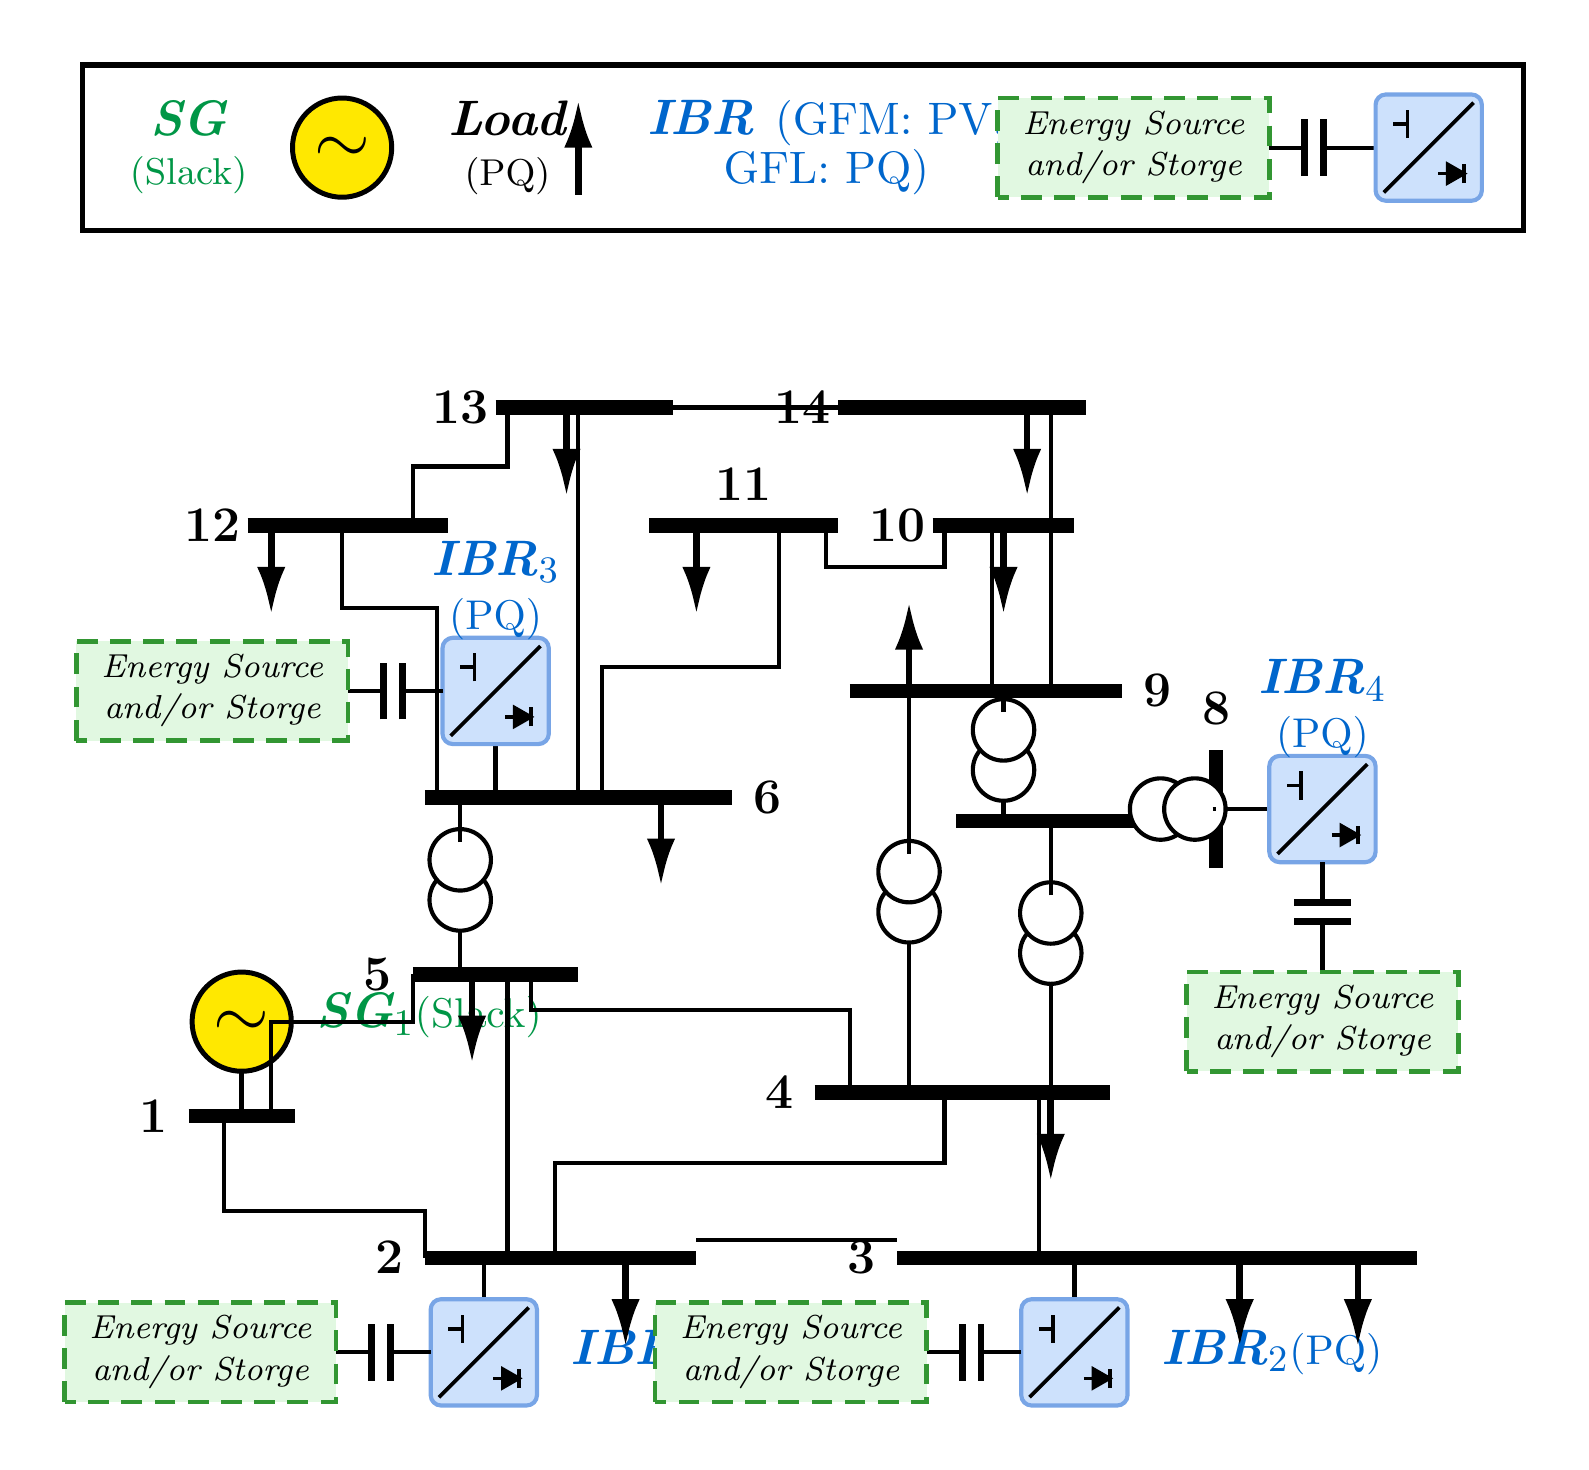
\includegraphics[width=0.82\textwidth]{ieee14_dual_mode_ibr_diagram.png}
\caption{ตำแหน่ง IBR แบบสองโหมดบนระบบ IEEE 14-bus}
\end{figure}

เมื่อเกิดการเปลี่ยนโหมด ระบบตรวจความต่อเนื่องของกระแสที่ terminal และแก้ algebraic right-limit ใหม่ก่อน commit state หลักการนี้ช่วยหลีกเลี่ยงการสร้าง current impulse เชิงตัวเลขให้กับ network และทำให้โหมด GFL/GFM ใช้โครงสร้าง state ที่ติดตามได้ตลอดการจำลอง

\templatesubheading{3. พัฒนา supervisor สำหรับเลือกและสลับโหมดอัตโนมัติ}
หลัง SG ถูกปลด supervisor จะประเมินความรุนแรงของ disturbance และสถานะของแหล่งอ้างอิง หากค่าดัชนีสูงกว่า threshold สำหรับเปิดใช้งาน GFM จะเพิ่มจำนวน IBR ที่ทำหน้าที่สร้างกริด และเมื่อระบบกลับเข้าสู่ช่วงปลอดภัยต่อเนื่องตาม dwell time จึงค่อยลดจำนวน GFM ลง กลไก hysteresis ใช้ threshold เปิดและปิดต่างกันเพื่อลดการสลับโหมดถี่เกินไป

ในช่วงที่ SG offline candidate ของ GFM ถูกคัดกรองด้วย equilibrium convergence, KCL, finite state, conditioning และ small-signal damping ก่อนนำไปใช้จริง อย่างไรก็ตาม linear screen เป็นเพียงเงื่อนไขเบื้องต้น จึงยังต้องยืนยันอีกครั้งจาก nonlinear time-domain simulation
\clearpage
\templatesubheading{4. ทดสอบเหตุการณ์ต่อเนื่องบนระบบ IEEE 14-bus}
กรณีทดสอบหลักมีระยะเวลา 250 วินาที ประกอบด้วยเหตุการณ์ที่กระทบทั้ง generation, load และ network topology เพื่อทดสอบการตัดสินใจของ supervisor ในหลายสภาวะ ดังตารางที่~\ref{tab:events}

\begin{table}[H]
\centering
\caption{ลำดับเหตุการณ์หลักของกรณีศึกษา}
\label{tab:events}
\begin{tabularx}{0.92\textwidth}{@{}r l X@{}}
\toprule
เวลา (s) & เหตุการณ์ & รายละเอียด \\
\midrule
20.000 & SG trip & ปลด SG ที่บัส 1 ออกจากระบบและเริ่มช่วงที่ต้องมี IBR ทำหน้าที่ voltage-forming \\
50.000 & Load step & เพิ่มโหลดเพื่อทดสอบความสามารถในการรองรับการเปลี่ยนสมดุลกำลัง \\
85.000--85.150 & Fault & เกิด fault ที่บัส 9 และเคลียร์ fault หลัง 0.15 s \\
110.000 & Line trip & ปลดสายส่ง 6--13 ทำให้ network topology เปลี่ยน \\
145.000 & Restore request & เริ่มกระบวนการคืน SG และถ่ายโอนผู้ถือมุมอ้างอิงกลับ \\
159.252 & SG reclose & SG กลับมาเชื่อมต่อสำเร็จจากผลของ adaptive arm \\
173.127 & Mode return & IBR กลับสู่โหมดหลัง handback สำเร็จ \\
250.000 & End of run & สิ้นสุดการจำลองโดยระบบกลับเข้าสู่สภาวะใกล้ steady state \\
\bottomrule
\end{tabularx}
\end{table}

รูปที่~\ref{fig:supervisor} แสดงดัชนีความรุนแรงของ IBR แต่ละตัว การเปลี่ยนโหมด และผู้ถือมุมอ้างอิงของระบบ จะเห็นว่าเมื่อ SG ถูกปลดที่ 20 s supervisor เปลี่ยน IBR บางตัวเป็น GFM เพื่อรักษาแหล่งอ้างอิงของโครงข่าย และเมื่อ SG กลับเข้าสู่ระบบแล้วจึงถ่ายโอนบทบาทกลับอย่างเป็นลำดับ
\begin{figure}[H]
\centering
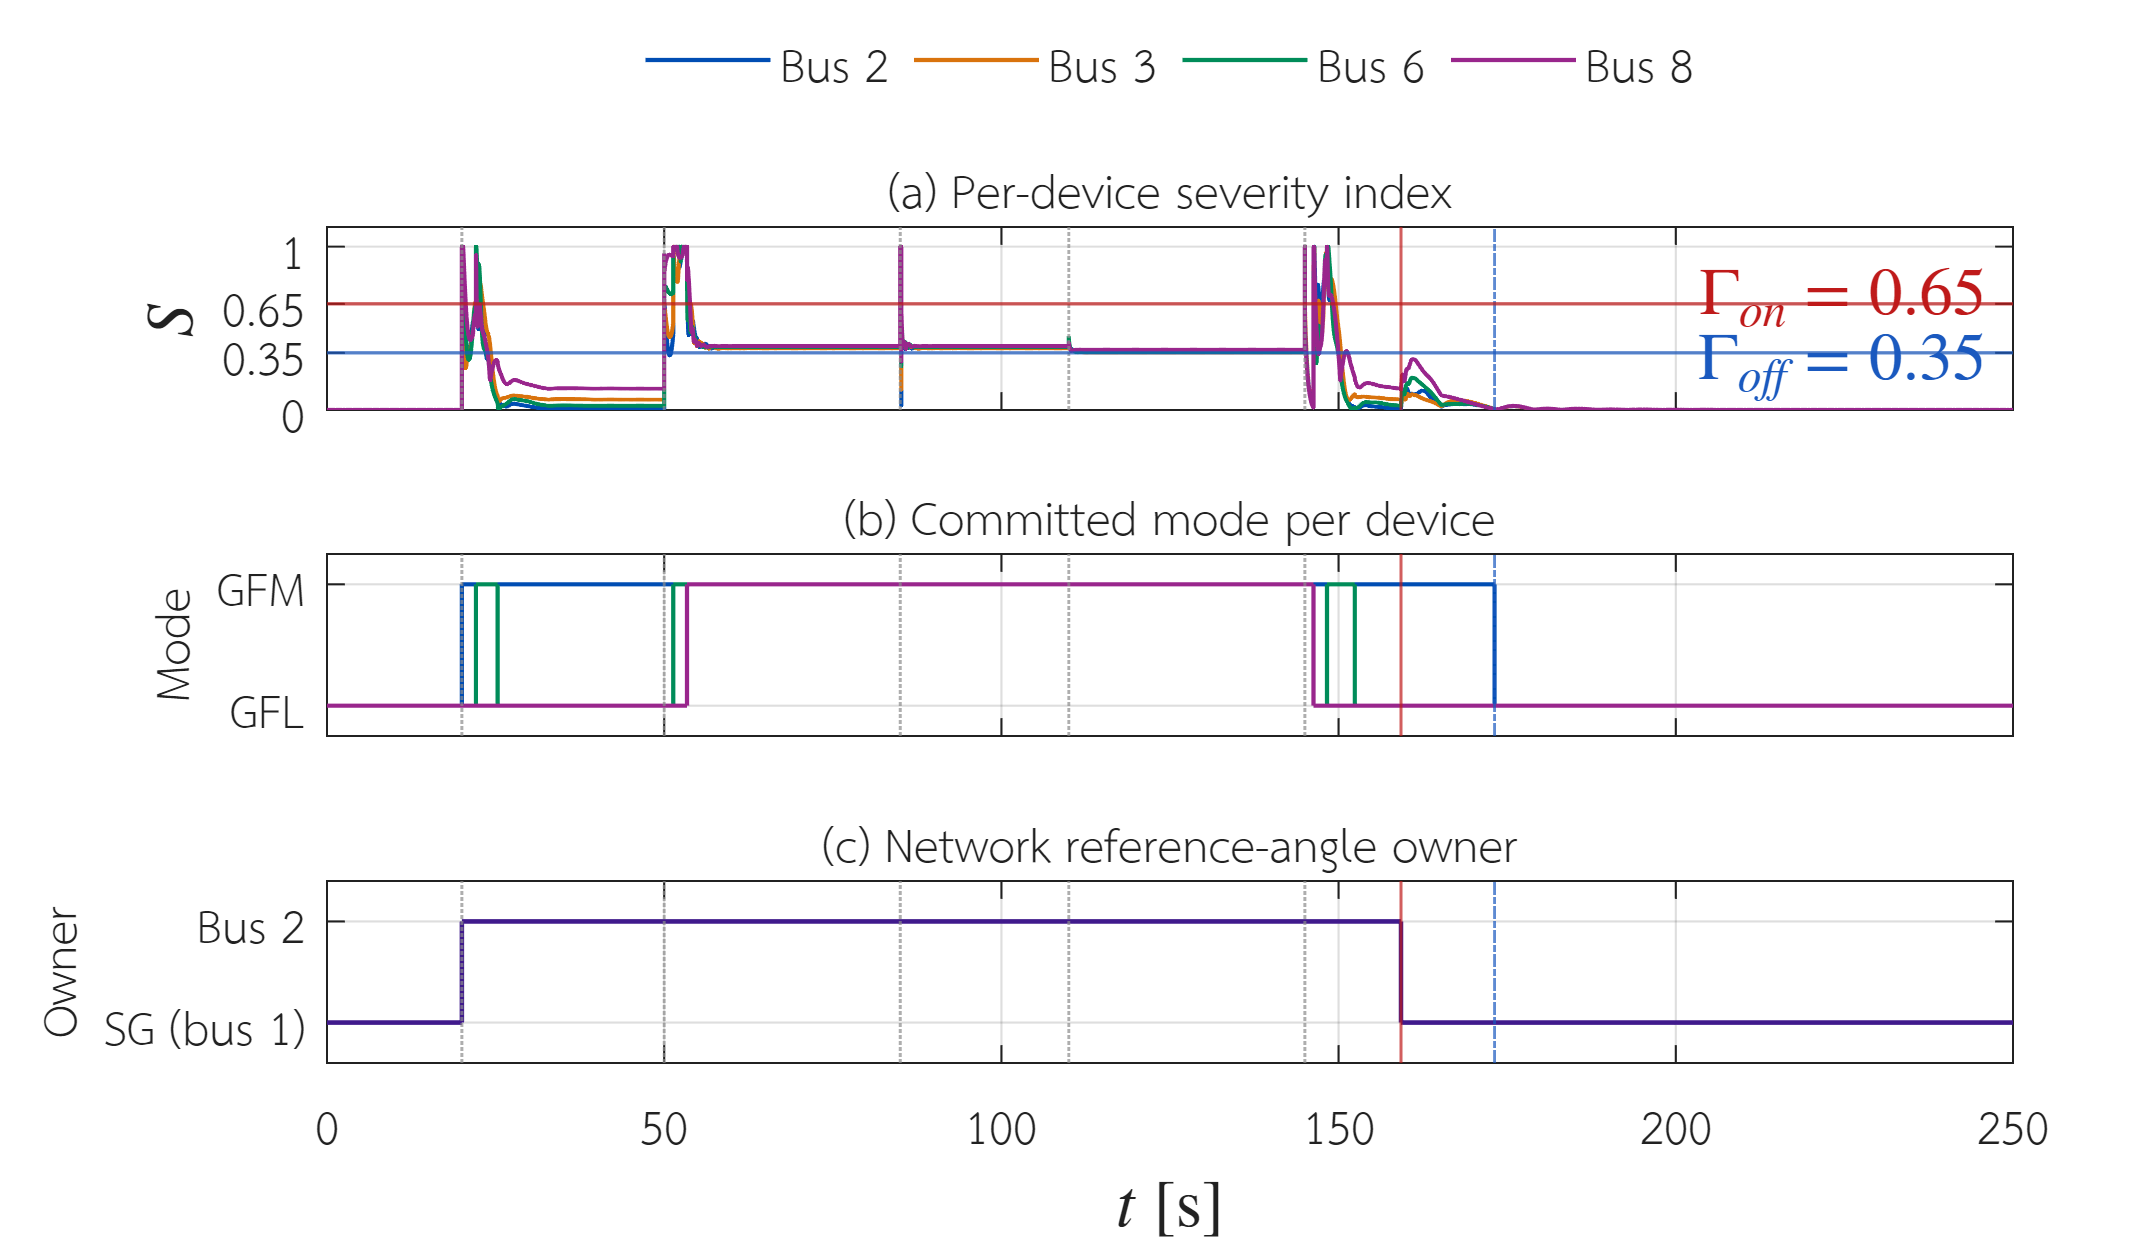
\includegraphics[width=0.94\textwidth]{fig_supervisor.png}
\caption{ดัชนีความรุนแรง การเปลี่ยนโหมด GFL/GFM และผู้ถือมุมอ้างอิงของระบบ}
\label{fig:supervisor}
\end{figure}

รูปที่~\ref{fig:electrical} แสดงกำลัง active/reactive ของอุปกรณ์ ความถี่เฉลี่ยของระบบ และแรงดันต่ำสุดของบัสตลอดเหตุการณ์ แม้มีการเปลี่ยน topology หลายครั้ง ระบบสามารถดำเนินการจำลองต่อไปจนถึง 250 s และหลังการคืน SG ค่าความถี่กลับมาใกล้ 60 Hz

\begin{figure}[H]
\centering
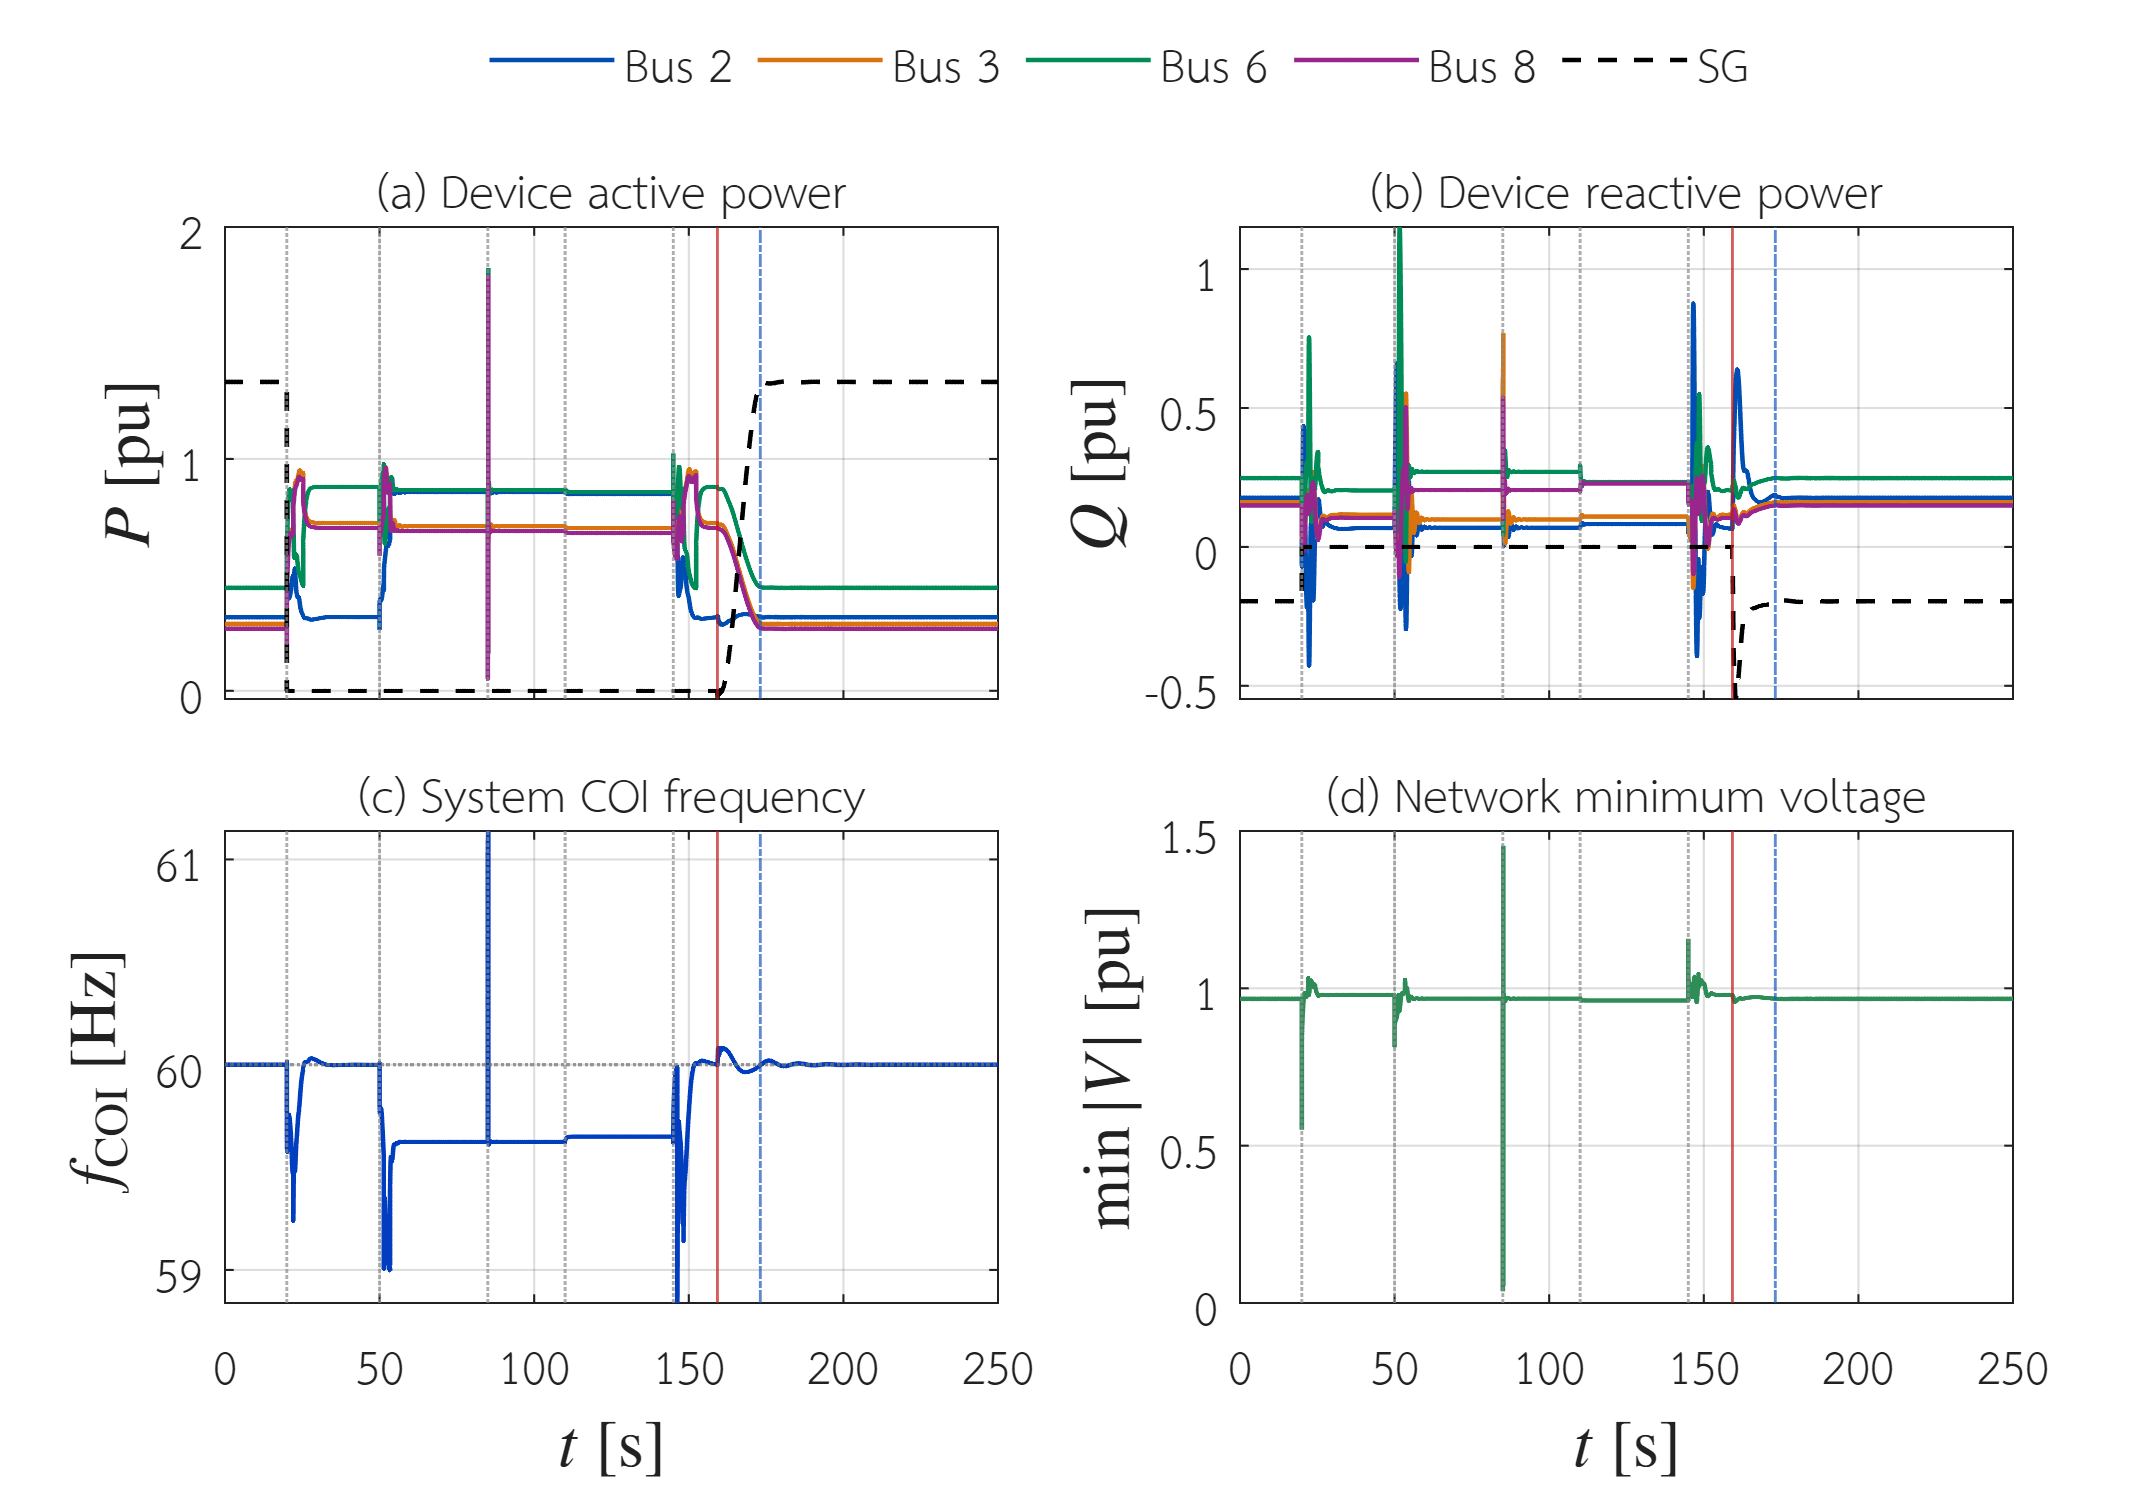
\includegraphics[width=0.96\textwidth]{fig_electrical.png}
\caption{ผลตอบสนองทางไฟฟ้าของ adaptive switching arm}
\label{fig:electrical}
\end{figure}

ค่าปลายทางของ adaptive arm ให้ความถี่ประมาณ \NewRunTerminalF\ และการจำลองเดินครบ \NewRunEnd\ วินาที โดยมี residual สุดท้ายเท่ากับ \NewRunResidual\ ผลดังกล่าวแสดงว่ากรอบการสลับโหมดสามารถประคองระบบผ่านลำดับเหตุการณ์ที่กำหนดและคืน SG เข้าสู่ระบบได้สำเร็จ

\clearpage
\templatesubheading{5. เปรียบเทียบนโยบายการควบคุม}
เพื่อประเมินผลของการสลับโหมดอัตโนมัติ โครงงานเปรียบเทียบ adaptive policy กับกรณีตรึงจำนวน GFM และกรณีปิดการสลับโหมด โดยใช้ event schedule เดียวกันและไม่ extrapolate ผลของแขนที่หยุดก่อนครบ horizon
\begin{table}[H]
\centering
\caption{สรุปผลนโยบายที่ใช้เปรียบเทียบ}
\begin{tabularx}{0.96\textwidth}{@{}l r l X@{}}
\toprule
นโยบาย & Horizon (s) & ผลการรัน & ข้อสังเกต \\
\midrule
Adaptive switching & \ArmAdaptiveHorizon & สำเร็จ & ปรับจำนวน GFM ตามสภาวะและคืน SG สำเร็จ \\
Pinned GFM = 1 & \ArmPinnedgfmOneHorizon & สำเร็จ & ใช้ GFM หนึ่งตัวตลอดช่วงที่กำหนด \\
Pinned GFM = 2 & \ArmPinnedgfmTwoHorizon & สำเร็จ & ใช้ GFM สองตัวตลอดช่วงที่กำหนด \\
Pinned GFM = 4 & \ArmPinnedgfmFourHorizon & หยุดก่อน horizon & ผ่าน linear screen แต่ nonlinear TS พบ minimum-step failure \\
Locked GFL & \ArmLockedgflHorizon & หยุดเมื่อ SG หาย & ไม่มี voltage-forming source หลัง SG trip \\
No adaptation & \ArmNoadaptationHorizon & สำเร็จ & ใช้ numerical step policy ที่ไม่ปรับแบบ adaptive \\
\bottomrule
\end{tabularx}
\end{table}

\begin{figure}[H]
\centering
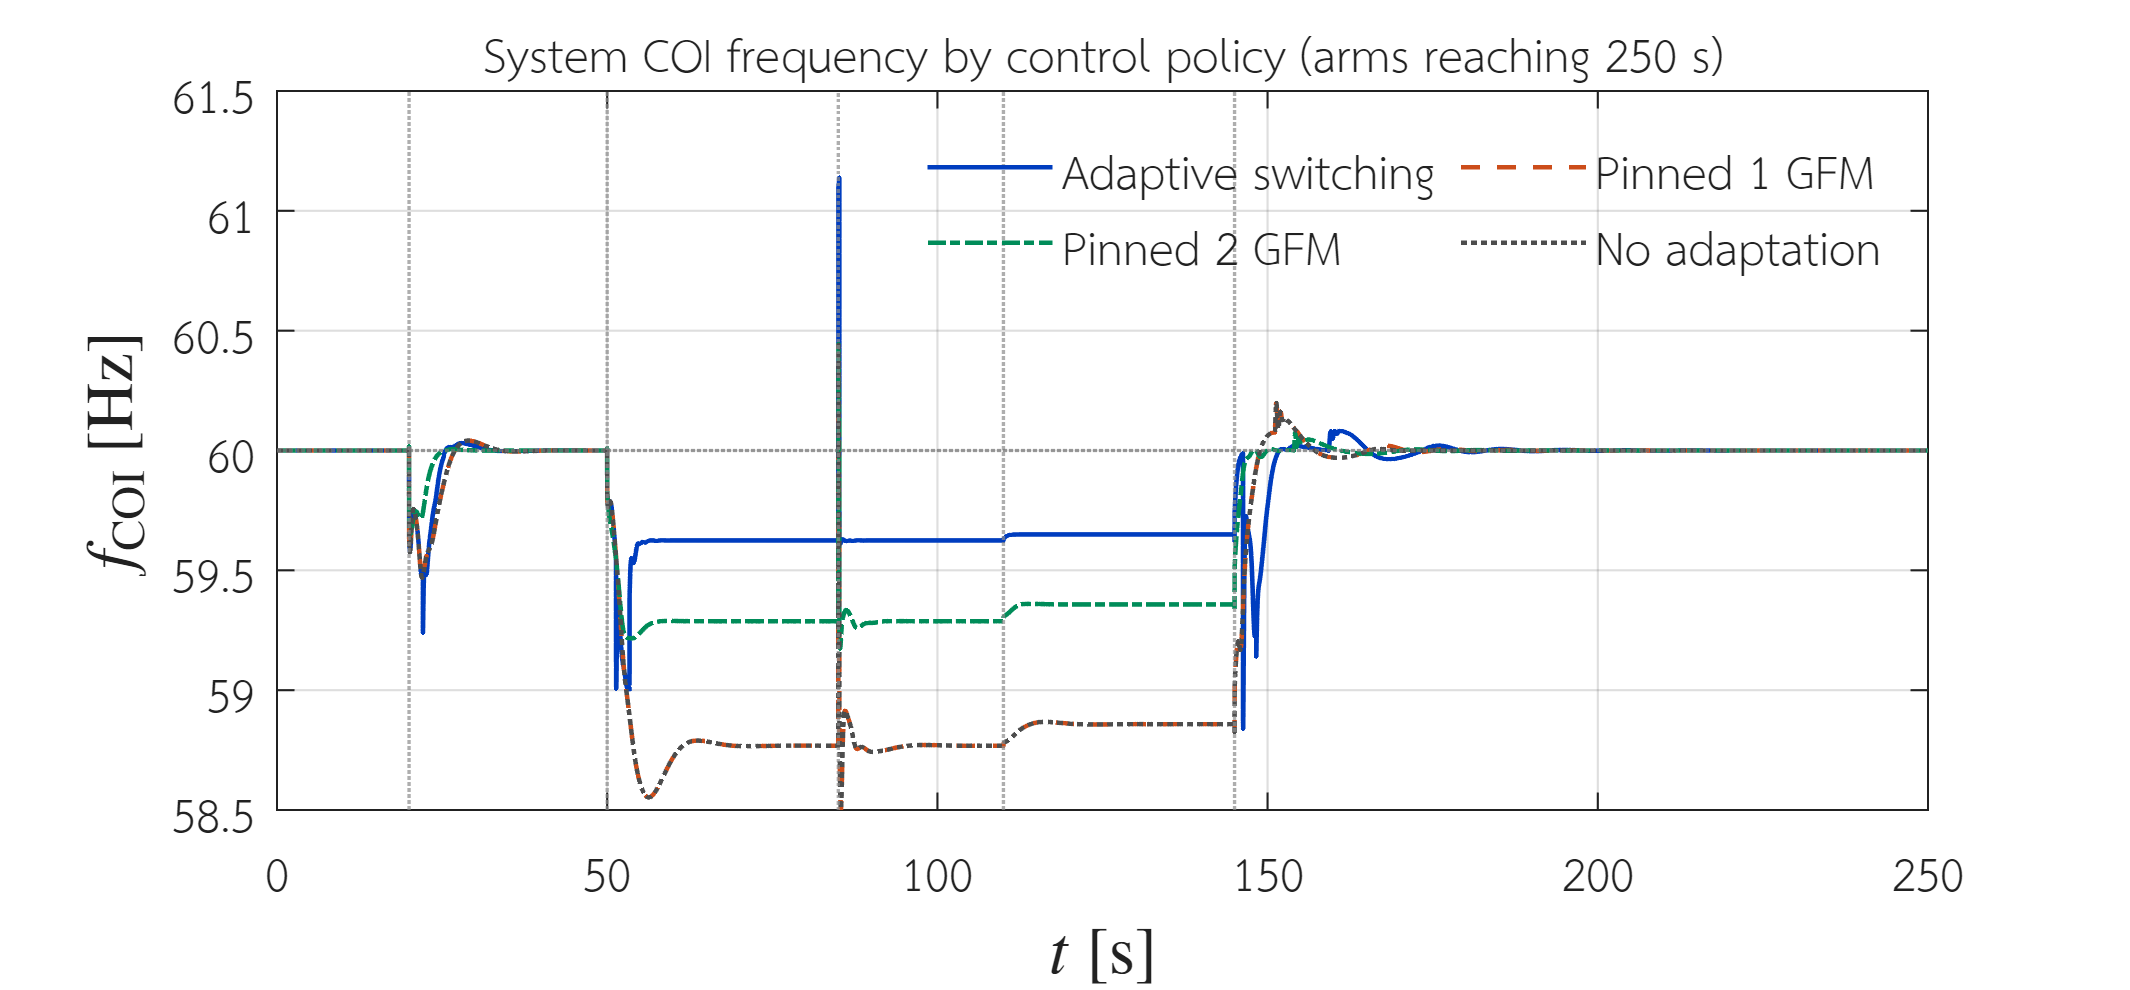
\includegraphics[width=0.94\textwidth]{fig_policy.png}
\caption{การเปรียบเทียบความถี่เฉลี่ยของระบบสำหรับนโยบายที่เดินถึง 250 s}
\end{figure}

ผลเปรียบเทียบชี้ให้เห็นว่าการมี GFM อย่างน้อยหนึ่งตัวหลัง SG trip เป็นเงื่อนไขจำเป็น แต่การเพิ่มจำนวน GFM สูงสุดไม่ได้รับประกันผล nonlinear ที่ดีกว่าเสมอ Adaptive policy จึงมีจุดเด่นที่ปรับระดับการสนับสนุนของ IBR ตาม disturbance และลดบทบาท GFM เมื่อระบบกลับสู่สภาวะปกติ

\templatesubheading{6. สรุปผลที่ได้รับจากโครงงาน}
โครงงานสามารถเชื่อม PF, SSSA และ TS เข้ากับ IBR แบบ dual-mode และ supervisor ในกรอบเดียวกันได้สำเร็จ กรณี adaptive เดินครบ 250 s ผ่านเหตุการณ์ SG trip, load step, fault, line trip และ SG restoration พร้อมรักษาเงื่อนไขการมีแหล่งอ้างอิงของระบบและตรวจ continuity ทุกครั้งที่เปลี่ยนโหมด ผลจาก pinned/locked policies ยังช่วยแสดงให้เห็นขอบเขตการทำงานและเหตุผลที่ต้องมีการตัดสินใจแบบอัตโนมัติแทนการกำหนดโหมดคงที่เพียงแบบเดียว
\clearpage
\templateheading{ประโยชน์ที่ได้รับจากโครงงาน}
\templatesubheading{ประโยชน์ด้านวิชาการและการพัฒนาแบบจำลอง}
\begin{enumerate}
\item ได้กรอบการจำลองระบบไฟฟ้ากำลังที่ใช้สมการและ state mapping ร่วมกันตั้งแต่ PF, equilibrium, SSSA จนถึง TS ทำให้ตรวจสอบความสอดคล้องของผลได้ง่ายขึ้น
\item ได้แบบจำลอง IBR ที่สามารถสลับระหว่าง GFL และ GFM ภายใน container เดียว โดยรักษา state ทางกายภาพที่สำคัญเมื่อเปลี่ยนโหมด
\item ได้แนวทางใช้ small-signal screening ร่วมกับ nonlinear time-domain validation เพื่อหลีกเลี่ยงการสรุปผลจาก eigenvalue เพียงอย่างเดียว
\item ได้ชุดกรณีศึกษา IEEE 14-bus ที่มีเหตุการณ์หลายชนิดสำหรับใช้ทดสอบงานด้าน IBR และการเปลี่ยนโหมดในอนาคต
\end{enumerate}

\templatesubheading{ประโยชน์ด้านการประยุกต์ใช้งาน}
\begin{enumerate}
\item แนวคิด supervisor สามารถใช้เป็นพื้นฐานในการศึกษาการจัดสรรบทบาท GFM เฉพาะช่วงที่ระบบต้องการ voltage-forming support แทนการกำหนดให้ converter ทุกตัวทำงานในโหมดเดียวตลอดเวลา
\item กรอบการทำงานช่วยศึกษาการถ่ายโอนผู้ถือมุมอ้างอิงระหว่าง SG และ IBR เมื่อระบบเกิด islanding หรืออยู่ในช่วง restoration
\item ผลการเปรียบเทียบนโยบายช่วยให้เห็น trade-off ระหว่างความมั่นคงของระบบ จำนวน IBR ที่ทำหน้าที่ GFM และความซับซ้อนของการควบคุม
\end{enumerate}

\templateheading{ปัญหาและอุปสรรคที่เกิดขึ้น}
\begin{enumerate}
\item หลัง SG trip ระบบไม่สามารถแก้สมการต่อได้หากไม่มี IBR อย่างน้อยหนึ่งตัวทำหน้าที่ voltage-forming เนื่องจากไม่มีแหล่งกำหนดมุมอ้างอิงของโครงข่าย
\item การสลับ GFL/GFM ทำให้ state order และ controller states เปลี่ยนบทบาท หาก map state ไม่ถูกต้องอาจเกิด discontinuity ของกระแสและทำให้ Newton corrector ไม่ลู่เข้า
\item candidate ที่ผ่าน SSSA ไม่ได้หมายความว่าจะผ่าน nonlinear TS เสมอ ตัวอย่างคือกรณีตรึง GFM ทั้ง 4 ตัวซึ่งผ่าน linear screen แต่หยุดก่อนครบ horizon
\item การจำลองแบบ implicit และ adaptive time step ใช้เวลาคำนวณสูง โดยเฉพาะช่วง fault หรือช่วงที่ topology เปลี่ยนและต้องแก้ nonlinear equations ซ้ำหลายครั้ง
\item ผลเปรียบเทียบกับโปรแกรมหรือเอกสารอ้างอิงบางชุดมีความต่างด้าน model, convention และ numerical method จึงต้องแยกผลที่ใช้เป็น primary validation ออกจากผลที่ใช้เป็น diagnostic
\end{enumerate}
\templateheading{แนวทางการแก้ไขปัญหาและอุปสรรคที่เกิดขึ้น}
\begin{enumerate}
\item กำหนด reference-owner guard ให้ระบบตรวจว่ามี SG หรือ GFM อย่างน้อยหนึ่งแหล่งก่อนเรียกตัวแก้สมการ หากไม่มีให้หยุดแบบ fail-closed แทนการฝืนคำนวณต่อ
\item ใช้ fixed superset state สำหรับ IBR และกำหนดขั้นตอน state transfer ที่ชัดเจน โดย carry plant states, initialize controller states จาก accepted operating point และตรวจ terminal-current continuity ก่อน commit
\item ใช้ SSSA เป็นเพียง screening ขั้นแรก และยืนยัน candidate ที่เลือกด้วย nonlinear TS ทุกครั้ง เพื่อไม่ให้ผลเชิงเส้นถูกตีความเกินขอบเขต
\item ใช้ implicit trapezoidal solver ร่วมกับ adaptive step control, exact event landing และ rollback ของ rejected step เพื่อลดปัญหาการลู่เข้าในช่วง disturbance รุนแรง
\item แยกแหล่งอ้างอิงภายนอกเป็น primary comparison และ diagnostic comparison พร้อมรายงานความต่างตามจริง ไม่ปรับ tolerance เพื่อให้ผลดูสอดคล้องเกินหลักฐาน
\end{enumerate}

\clearpage
\templateheading{โครงงานที่คาดว่าจะดำเนินการต่อไป}
\begin{enumerate}
\item ขยายจาก balanced RMS model ไปสู่ unbalanced network และ electromagnetic transient (EMT) เพื่อศึกษาพฤติกรรม converter และ protection ในช่วงเวลาที่เร็วขึ้น
\item เพิ่มแบบจำลอง protection, current limiting, fault ride-through และข้อกำหนด grid code เพื่อให้กรณีศึกษาสะท้อนข้อจำกัดของอุปกรณ์จริงมากขึ้น
\item ทดสอบกรอบการเลือก GFM บนระบบขนาดใหญ่กว่า IEEE 14-bus และกรณีที่มี IBR จำนวนมาก เพื่อประเมิน scalability ของ candidate selection และ supervisor
\item พัฒนาเกณฑ์เลือก candidate ให้พิจารณาทั้ง damping, voltage support, converter loading, energy reserve และต้นทุนการสลับโหมดร่วมกัน
\item เชื่อมต่อแบบจำลองกับ hardware-in-the-loop หรือ controller prototype เพื่อทดสอบการเปลี่ยนโหมดและ handback ภายใต้ข้อจำกัดของระบบควบคุมจริง
\end{enumerate}

\vfill
\begin{center}
\fbox{\begin{minipage}{0.90\textwidth}
\centering
เอกสารฉบับนี้จัดรูปแบบเป็น “เอกสารสรุปวิชาโครงงาน” โดยเน้นวัตถุประสงค์ ที่มาของปัญหา วิธีดำเนินงาน ผลที่ได้รับ ประโยชน์ ปัญหา/แนวทางแก้ และงานที่จะดำเนินการต่อไป ตามลำดับของเอกสารตัวอย่าง
\end{minipage}}
\end{center}

\end{document}
